% Options for packages loaded elsewhere
\PassOptionsToPackage{unicode}{hyperref}
\PassOptionsToPackage{hyphens}{url}
%
\documentclass[
]{article}
\usepackage{amsmath,amssymb}
\usepackage{iftex}
\ifPDFTeX
  \usepackage[T1]{fontenc}
  \usepackage[utf8]{inputenc}
  \usepackage{textcomp} % provide euro and other symbols
\else % if luatex or xetex
  \usepackage{unicode-math} % this also loads fontspec
  \defaultfontfeatures{Scale=MatchLowercase}
  \defaultfontfeatures[\rmfamily]{Ligatures=TeX,Scale=1}
\fi
\usepackage{lmodern}
\ifPDFTeX\else
  % xetex/luatex font selection
\fi
% Use upquote if available, for straight quotes in verbatim environments
\IfFileExists{upquote.sty}{\usepackage{upquote}}{}
\IfFileExists{microtype.sty}{% use microtype if available
  \usepackage[]{microtype}
  \UseMicrotypeSet[protrusion]{basicmath} % disable protrusion for tt fonts
}{}
\makeatletter
\@ifundefined{KOMAClassName}{% if non-KOMA class
  \IfFileExists{parskip.sty}{%
    \usepackage{parskip}
  }{% else
    \setlength{\parindent}{0pt}
    \setlength{\parskip}{6pt plus 2pt minus 1pt}}
}{% if KOMA class
  \KOMAoptions{parskip=half}}
\makeatother
\usepackage{xcolor}
\setlength{\emergencystretch}{3em} % prevent overfull lines
\providecommand{\tightlist}{%
  \setlength{\itemsep}{0pt}\setlength{\parskip}{0pt}}
\setcounter{secnumdepth}{-\maxdimen} % remove section numbering
\usepackage[margin=1in]{geometry}
\usepackage[most]{tcolorbox}
\usepackage{graphicx}
\definecolor{taskgreen}{HTML}{4CAF50}
\ifLuaTeX
  \usepackage{selnolig}  % disable illegal ligatures
\fi
\IfFileExists{bookmark.sty}{\usepackage{bookmark}}{\usepackage{hyperref}}
\IfFileExists{xurl.sty}{\usepackage{xurl}}{} % add URL line breaks if available
\urlstyle{same}
\hypersetup{
  hidelinks,
  pdfcreator={LaTeX via pandoc}}

\author{}
\date{}

\begin{document}

\begin{center}
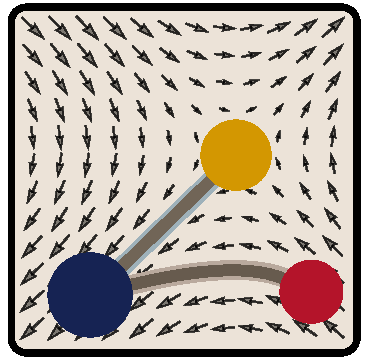
\includegraphics[width=0.5\textwidth]{img/favicon.pdf}
\end{center}
\vspace{1em}

\begin{center}
{\Huge\bfseries Mathematical modelling in ecology and evolution (EEB314/1430)}
\end{center}
\vspace{1em}

Mathematics is central to science because it provides a rigorous way to
go from a set of assumptions to their logical consequences. In ecology
\& evolution this might be how we think a virus will spread and evolve,
how climate change will impact a threatened population, or how much
genetic diversity we expect to see in a randomly mating population. In
this course you'll learn how to build, analyze, and interpret
mathematical models of increasing complexity through readings, lectures,
labs, and a final project. Our focus is on deterministic dynamical
models (recursions and differential equations), which requires us to use
and learn some calculus and linear algebra.

Please see the
\href{https://artsci.calendar.utoronto.ca/course/eeb314h1}{University of
Toronto Academic Calendar} for more details on the course prerequisites
and additional information on the distribution/breadth requirements this
course satisfies.

Next taught: Fall 2026

Previously taught: Fall 2025, Fall 2024, Fall 2022 (EEB430), Fall 2021
(EEB430)

\clearpage

\hypertarget{instructors}{%
\section{Instructors}\label{instructors}}

\hypertarget{professor}{%
\subsection{Professor}\label{professor}}

Matthew Osmond (he/him)

\begin{itemize}
\tightlist
\item
  email: mm.osmond@utoronto.ca
\item
  office: Earth Sciences (ES) room 3041
\item
  website: \href{https://osmond-lab.github.io/}{osmond-lab.github.io}
\end{itemize}

\hypertarget{teaching-assistant}{%
\subsection{Teaching assistant}\label{teaching-assistant}}

Mete Yukel (they/he)

\begin{itemize}
\tightlist
\item
  email: mete.yuksel@mail.utoronto.ca
\end{itemize}

\hypertarget{when-and-where}{%
\section{When and where}\label{when-and-where}}

\hypertarget{lectures}{%
\subsection{Lectures}\label{lectures}}

\begin{itemize}
\tightlist
\item
  Monday 10:10 - 11:00 AM, Earth Sciences (ES) room 3087
\item
  Wednesday 10:10 - 11:00 AM, Earth Sciences (ES) room 3087
\end{itemize}

\hypertarget{labs}{%
\subsection{Labs}\label{labs}}

\begin{itemize}
\tightlist
\item
  Wednesday, 3:10 - 5:00 PM, Earth Sciences (ES) room 3087
\end{itemize}

\hypertarget{course-structure}{%
\section{Course structure}\label{course-structure}}

\hypertarget{learning-objectives}{%
\subsection{Learning objectives}\label{learning-objectives}}

\begin{itemize}
\tightlist
\item[$\textcolor{taskgreen}{\boxed{\checkmark}}$]
  build a model: go from a verbal description of a biological system to
  a set of equations
\item[$\textcolor{taskgreen}{\boxed{\checkmark}}$]
  analyze a model: manipulate a set of equations into a mathematical
  expression of interest
\item[$\textcolor{taskgreen}{\boxed{\checkmark}}$]
  interpret a model: translate mathematical expressions back into
  biological meaning
\end{itemize}

\hypertarget{weekly-tasks}{%
\subsection{Weekly tasks}\label{weekly-tasks}}

\begin{itemize}
\tightlist
\item[$\textcolor{taskgreen}{\boxed{\checkmark}}$]
  attend two lectures (2h)
\item[$\textcolor{taskgreen}{\boxed{\checkmark}}$]
  participate in one lab (2h)
\item[$\textcolor{taskgreen}{\boxed{\checkmark}}$]
  do practice problems (listed at end of each lecture)
\item[$\textcolor{taskgreen}{\boxed{\checkmark}}$]
  read assigned portions of the text (when more info needed)
\end{itemize}

\hypertarget{grading-scheme}{%
\subsection{Grading scheme}\label{grading-scheme}}

\begin{itemize}
\tightlist
\item
  in-class tests: 4 x 20\% (4 x 15\% for grad students)
\item
  final project: 20\% (40\% for grad students)
\end{itemize}

\hypertarget{textbook}{%
\section{Textbook}\label{textbook}}

Otto \& Day 2007. \href{https://www.zoology.ubc.ca/biomath/}{A
biologist's guide to mathematical modeling in ecology and evolution}.

\begin{itemize}
\tightlist
\item
  \href{https://librarysearch.library.utoronto.ca/permalink/01UTORONTO_INST/14bjeso/alma991106921343406196}{UofT
  library e-copies}
\item
  \href{https://librarysearch.library.utoronto.ca/permalink/01UTORONTO_INST/14bjeso/alma991106624476006196}{UofT
  library physical-copies}
\item
  \href{https://press.princeton.edu/books/hardcover/9780691123448/a-biologists-guide-to-mathematical-modeling-in-ecology-and-evolution}{buy
  your own copy}
\end{itemize}

\hypertarget{final-project}{%
\section{Final project}\label{final-project}}

\hypertarget{construct-your-own-model}{%
\subsection{Construct your own model}\label{construct-your-own-model}}

In this project you will use the tools you've learned in class and apply
them to a model that you develop. The model can be about any phenomenon
in ecology and evolution, as long as you make up the model. I suggest
you stick with dynamical models and analyses learned in class.

You'll do the final project in two parts.

\begin{itemize}
\tightlist
\item[$\textcolor{taskgreen}{\boxed{\checkmark}}$]
  Part 1 (25\%)

  \begin{itemize}
  \tightlist
  \item
    State your biological question
  \item
    Describe your model in words (ie, the main assumptions) and,
    optionally, with a diagram (eg, flow diagram or life cycle)
  \item
    Write down the equations that you plan to analyze
  \item
    Describe what analysis you plan to do and how this will answer your
    question
  \item
    Max 500 words
  \end{itemize}
\item[$\textcolor{taskgreen}{\boxed{\checkmark}}$]
  Part 2 (75\%)

  \begin{itemize}
  \tightlist
  \item
    Motivate and state your biological question
  \item
    Describe your model assumptions in detail, defining all parameters
    and variables
  \item
    Write down the equations for your model
  \item
    Analyze your model
  \item
    Explain how the results address your original question
  \item
    Suggest how the model could be improved or extended
  \item
    Plots and supplementary Jupyter notebooks welcome but not required
  \item
    Max 2000 words (4000 for grad students)
  \end{itemize}
\end{itemize}

\begin{tcolorbox}[breakable,colback=cyan!8,colframe=cyan!65!black,title=Class presentations,fonttitle=\bfseries]
Grad students will also present their final project in class. Everyone
may be asked to give a 2m lightning presentation on part 1.\end{tcolorbox}

\begin{tcolorbox}[breakable,colback=green!8,colframe=green!65!black,title=Tip,fonttitle=\bfseries]
If you are having trouble coming up with a new model, take one of the
models that we've analysed in the course and change one or more of its
underlying assumptions to get a new set of equations. Then analyse these
equations. Discuss the differences between the assumptions used and also
between the results obtained.\end{tcolorbox}

\begin{tcolorbox}[breakable,colback=red!8,colframe=red!65!black,title=AI policy,fonttitle=\bfseries]
Your final project must be conducted and submitted individually. That
said, you are encouraged to discuss your ideas and analyses with others
as a way to shape and improve them. Your submitted work must, however,
reflect your own understanding and conclusions.

Similarly, use of artificial intelligence (AI) tools, such as ChatGPT,
Claude, Copilot, DeepL, Gemini, Google Translate, Grammarly, Llama,
etc., is allowed only to the extent that it aids your learning and
understanding. Any use of AI must cite the tool using APA guidelines and
specify exactly how AI was used, including the search term, the chat
history link (if available), and how the results were used. In cases
where a chat history is not available, please save a copy of the chat to
your computer in case we ask for more details. Again, your submitted
work must reflect your own understanding and conclusions. Getting AI
help to learn how to improve your grammar or to debug code or to check
an answer is appropriate in this course (if cited); having AI solve
problems for you or suggest ideas for a course project would not be
acceptable as then your submitted work cannot be your own. If in doubt,
please ask!\end{tcolorbox}

\clearpage
\vspace*{\fill}
\begin{center}
\Large See \url{https://osmond-lab.github.io/eeb314} for more info
\end{center}
\vspace*{\fill}

\end{document}
